\chapter{Steganografie}
Die Steganografie bezeichnet eine weitere Methode die Vertraulichkeit eines
Kommunikationsaustausches zu gewährleisten.
Es wird das Ziel verfolgt, eine Nachricht in einer für den Computer
zugänglichen Trägerdatei (engl. \textit{cover media}) zu verstecken, sodass eine
weitere Person die Existenz
einer geheimen Botschaft gar nicht erst vermuten würde. Eine Trägerdatei, unempfindlich
gegenüber kleinen Änderungen in den Daten eignet sich besonders gut für die
Anwendung steganografischer Verfahren. Digitale Bilddateien sowie Audio- und Videodateien
sind sehr geeignete Trägermedien,
da ihre Daten ein ganz natürliches Rauschen aufweisen.
In diesem Kapital soll ein Algorithmus vorgestellt werden, welcher
eine beliebig lange Nachricht in einem Bild versteckt und versucht,
die visuelle Qualität des Urbilds zu bewahren.

\section{Modifikation von Bilddateien}
Eine digitale Bilddatei besteht aus einer zweidimensionalen Anordnung von Pixel, wobei
jeder eine bestimmte Farbe annehmen kann. Farben können unterschiedlich
dargestellt werden, dass in der Bildwiedergabe am häufigsten verwendete Modell ist
der RGB-Farbraum. Die Farbwahrnehmung des menschlichen Auges kann durch
das additive Mischen der drei Grundfarben Rot, Grün und Blau (RGB)
nachgebildet werden \parencite[32-40]{BOOK:VC}. In computerorientierten Anwendungen
werden hierfür pro Farbkanal Zahlenwerte zwischen 0 und 255 gespeichert.
Je größer der Wert desto heller die Farbe, die Kombinationen
$(255,0,0)$, $(0,255,0)$ und $(0,0,255)$ beschreiben jeweils die Grundfarben Rot, Grün und Blau.
Das Mischen aller Farben $(255,255,255)$ ergibt Weiß und das Hinzufügen gar keines
Lichts $(0,0,0)$ resultiert in Schwarz. Kombinationen mit gleicher Intensität
$(100,100,100)$ werden als Grauton wahrgenommen. Pro Pixel müssen in einem Bild
also 3 Byte an Information gespeichert.
\begin{figure}[t]
  \centering
  \begin{minipage}[t]{0.3\textwidth}
    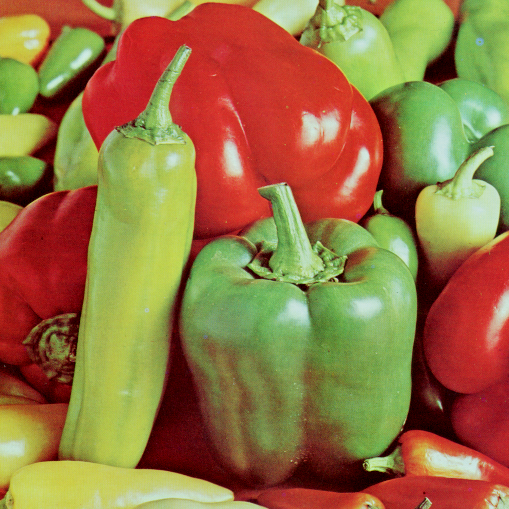
\includegraphics[width=1\textwidth]{peppers-0.png}
    \caption*{(a)}
  \end{minipage}
  \hfill
  \begin{minipage}[t]{0.3\textwidth}
    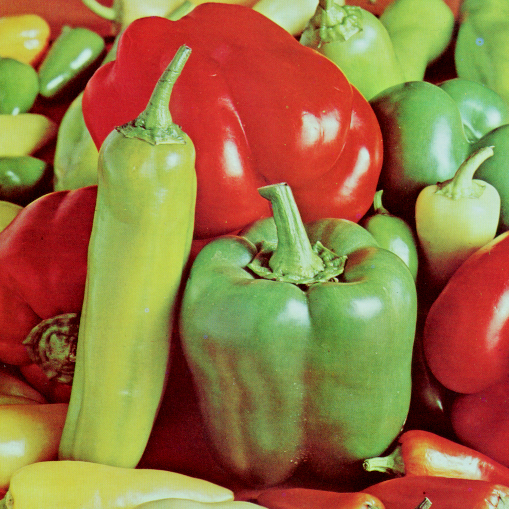
\includegraphics[width=1\textwidth]{peppers-1.png}
    \caption*{(b)}
  \end{minipage}
  \hfill
  \begin{minipage}[t]{0.3\textwidth}
    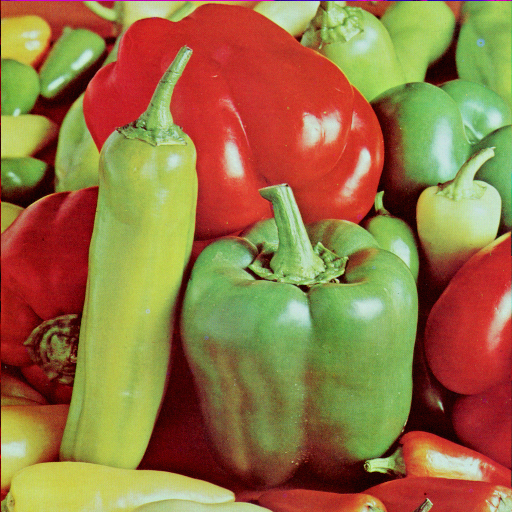
\includegraphics[width=1\textwidth]{peppers-2.png}
    \caption*{(c)}
  \end{minipage}%
  \vspace{0.5cm}
  \begin{minipage}[t]{0.3\textwidth}
    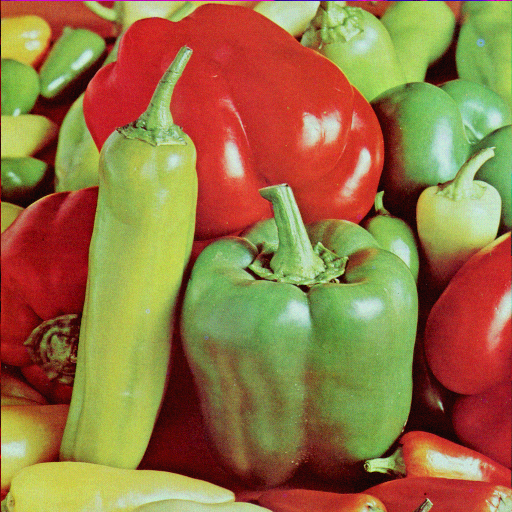
\includegraphics[width=1\textwidth]{peppers-3.png}
    \caption*{(d)}
  \end{minipage}
  \hfill
  \begin{minipage}[t]{0.3\textwidth}
    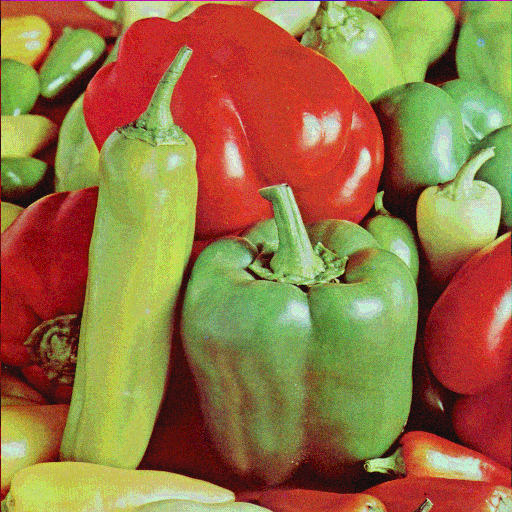
\includegraphics[width=1\textwidth]{peppers-4.png}
    \caption*{(e)}
  \end{minipage}
  \hfill
  \begin{minipage}[t]{0.3\textwidth}
    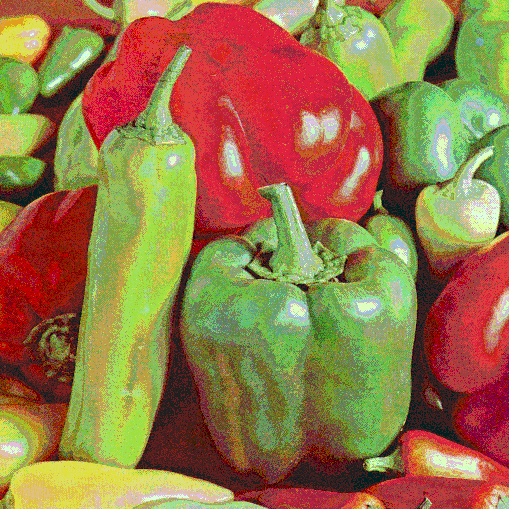
\includegraphics[width=1\textwidth]{peppers-5.png}
    \caption*{(f)}
  \end{minipage}%
  \vspace{0.5cm}
  \begin{minipage}[t]{0.3\textwidth}
    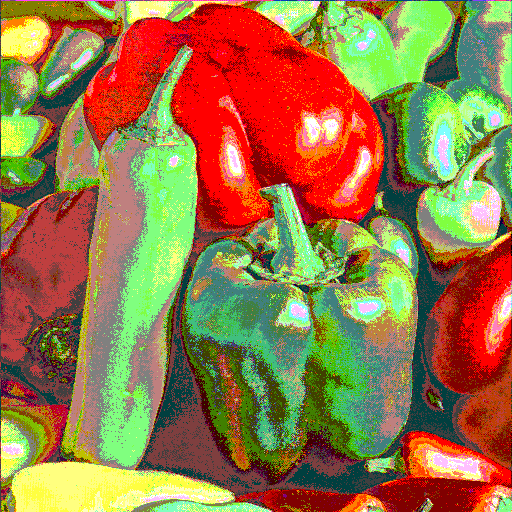
\includegraphics[width=1\textwidth]{peppers-6.png}
    \caption*{(g)}
  \end{minipage}
  \hfill
  \begin{minipage}[t]{0.3\textwidth}
    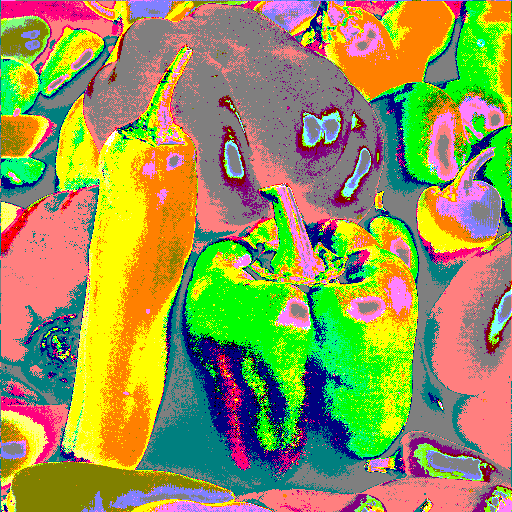
\includegraphics[width=1\textwidth]{peppers-7.png}
    \caption*{(h)}
  \end{minipage}
  \hfill
  \begin{minipage}[t]{0.3\textwidth}
    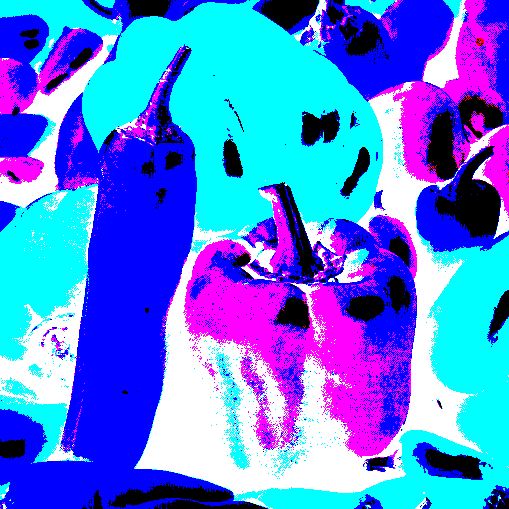
\includegraphics[width=1\textwidth]{peppers-8.png}
    \caption*{(i)}
  \end{minipage}
  \caption{Test}
\end{figure}
